%
%%%%%%%%%%%%%%%%%%%%%%%%%%%%%%%%%%%%%%%%%%%%%%%%%%%
%
%  E N T W I C K L U N G S U M G E B U N G
%
%%%%%%%%%%%%%%%%%%%%%%%%%%%%%%%%%%%%%%%%%%%%%%%%%%%
\chapter{Grundlagen}
\label{cha:grundlagen}
%
%
In dem Grundlagenkapitel geht es um das Basiswissen, auf dem die Arbeit aufbaut. Es wird näher auf die verwendeten Technologien eingegangen. Dabei werden die Frontend-Frameworks beleuchtet sowie die 3D Bibliotheken. Näher wir auch auf die Begriffe Resposive Webdesign, Usability und Performance eingegangen.
%
%
%%%%%%%%%%%%%%%%%%%%%%%%%%%%%%%%%%%%%%%%%%%%%%%%%%%
%
% S P A
%
%%%%%%%%%%%%%%%%%%%%%%%%%%%%%%%%%%%%%%%%%%%%%%%%%%%
%
\section{Single Page Anwendungen}
\label{sec:spa}
%
Früher war es bei Webanwendungen wichtig, soviel wie möglich auf dem Server zu erledigen. Bei modernen Webframeworks gilt jedoch genau das Gegenteil. Es wird versucht möglichst viel clientseitig umzusetzten.\textit{\glqq Dies steigert die Benutzerfreundlichkeit und schafft die Möglichkeit der Anpassung an die Auflösungen und Formfaktoren der vielen unterschiedlichen klassischen und mobilen Plattformen.\grqq } \cite{bahor_html5/webgl_2013}. Im Folgenden wird nun kurz etwas genauer darauf eingegangen was André Krämer in seinem Videokurs sehr gut und einfach erklärt hat.
%
\paragraph{Klassische Webanwendungen}
%
Bevor man sich damit befasst was Single Page Anwendungen sind, sollte man sich das Prinzip einer klassischen Webanwendung anschauen. Nehmen wir beispielsweise an, ein Client sendet eine Anfrage an einen Server. Hierbei handelt es sich um einen Webbrowser, welcher eine Webadresse öffnen möchte. Der Zielserver übernimmt die Verarbeitung. In der Regel laufen nun Skripte auf dem Server, welche HTML rendern. Schließlich bekommt der Client auf seine Anfrage eine Antwort in Form eines HTML-Dokumentes und kann es dann anzeigen. Bei diesem Vorgang liegt die komplette Verarbeitung bei dem Server. Der Webbrowser dient lediglich der Darstellung und einfachen Eingabe. Das die Daten auf einem Server verarbeitet werden wird deutlich, wenn ein Seitenwechsel vorgenommen wird. Dabei wird kurze Zeit nichts angezeigt während die Seite komplett neu lädt.\\
Mit der Einführung von AJAX\footnote{Ajax bzw. AJAX steht als Akronym für „Asynchronous JavaScript and XML“. Die Technologie ermöglicht es, einzelne Teile einer Webseite bei Bedarf asynchron zu laden, so dass sie dynamisch wird. Der angezeigte Inhalt lässt sich gezielt so manipulieren, ohne die komplette Seite neu zu laden.} in 2005 machte die Webentwicklung einen Schritt nach vorne. Nun war es nämlich möglich, Daten asynchron an den Server zu senden. Das heißt, der Server verabreitet zwar immer noch die Daten, sendet nun aber nur noch einen Teil des vorgerenderten Dokuments oder sogar nur einzelne Daten der Seite. Somit wird die Seite nicht wieder komplett neu geladen. Wenn man nun aber in einen komplett andern Bereich der Seite wechseln will, hilft AJAX nicht. Die Seite wird neu geladen und es dauert einen kurzen Moment bis das Ergebnis vom Webbrowser angezeigt werden kann. Um dieses Problem zu lösen, kommen \textit{Single Page Anwendungen} zum Einsatz.
\paragraph{Dezentralisierung der Webanwendung}
%
Im Grunde arbeiten SPA's nach folgendem Prinzip: Der Webbrowser sendet eine Anfrage an den Server. Dieser verarbeitet, wie bei klassischen Webanwendungen nun die Anfrage. Anschließend wird im Webbrowser eine Benutzeroberfläche dargestellt. Nun kommt der entscheidende Unterschied zu klassischen Anwendungen. Bei einem Seitenwechsel oder anderen Interaktionen des Benutzers wird eine neue Benutzeroberfläche erzeugt, indem Teile der Seite ausgetauscht werden. Die Seite wird nie komplett neu geladen. Der Nutzer bleibt immer auf der einen Seite, zumindest fühlt es sich für den Benutzer so an. Dieses Prinzip kennt der Anwender von Desktop-Anwendungen. Man hat sogar die Möglichkeit die Anwendung (zumindest teilweise) offlinefähig zu machen.\\
Die Grundlage einer solchen Anwendung ist das Routing. Abhängig vom Pfad werden bestimmte Bausteine der Anwendung angezeigt bzw. ausgeblendet. Wie wir im späteren Verlauf dieser Arbeit noch sehen werden, hat man tatsächlich nur eine HTML-Datei, welche abhängig vom Kontext immer andere Inhalte anzeigen kann.\\
%
Zusammenfassend lässt sich also festhalten, das ein Ziel von SPAs ist, die Kommunikation zwischen Client und Server enorm zu reduzieren. Um dies zu erreichen wird die Anwendung dezentralisiert. Das heißt, es gibt nur ein HTML Dokument\cite{domin_was_2018}. Durch den Einsatz von Frameworks, wie Angular, ist es möglich Inhalte zu aktualisieren oder zu einer anderen Seite zu wechseln, ohne die Seite über den Server neu zu laden.
\footnote{Das Prinzip von Single Page Anwendungen wird zum Beispiel von Googles Gmail und Gmaps sowie von Twitter verwendet}
%
%
%%%%%%%%%%%%%%%%%%%%%%%%%%%%%%%%%%%%%%%%%%%%%%%%%%%
%
% A U F B A U 
%
%%%%%%%%%%%%%%%%%%%%%%%%%%%%%%%%%%%%%%%%%%%%%%%%%%%
%
\section{Framework Angular}
\label{sec:angular7}
Das Framework Angular ist sehr umfangreich. Im Folgenden werden einige Grundlagen erläutert, die zur Implementierung einer Anwendung mit Angular benötigt werden. Dabei soll ein Grundverständis vermittelt werden, wie das Framework aufgebaut ist und wie es arbeitet.
\subsection{Komponentenbasierte Programmierung}
%
Angular ist ein Framework, das auf Komponenten setzt. Das Prinzip der komponentenbasierten Entwicklung kommt nicht nur bei Angular vor, sondern auch bei vielen anderen Programmiersprachen und Frameworks. Was in Angular Komponenten sind wird in dem Buch \textit{Angular: Grundlagen, fortgeschrittene Techniken und Best Practices mit TypeScript - ab Angular 4, inklusive NativeScript und Redux} folgendermaßen beschrieben:\\
%

\textit{\glqq Komponenten sind die Grundbausteine einer Angular Anwendung. Jede Anwendung ist aus vielen verschiedenen Komponenten zusammengesetzt, die jeweils eine bestimmte Aufgabe erfüllen. Eine Komponente beschreibt somit immer einen kleinen Teil der Anwendung, z. B. eine Seite oder ein einzelnes UI-Element.\grqq }\cite{woiwode_angular:_2017} \\

%
Im Grunde ist eine Komponente also nichts anderes als ein selbstdefinierter HTML-Knoten, den man im HTML Kontext ganz normal nutzen kann. Man erzeugt einfach DOM-Elemente\footnote{Wenn eine Webseite geladen wird, erstellt der Browser eine Document Object Model der Seite. Das HTML-DOM-Modell ist als Baum von Objekten aufgebaut. Diese Objekte sind ein der Regel einfache HTML-Tags} und kann sie dann automatisch in Angular nutzen.
Eine Komponente in Angular ist in drei Parts aufgeteilt: Logik, Vorlage und Style. Die Logik beschreibt die TypeScript Klassen, Eigenschaften, Methoden und so weiter. Sie beschreibt also, was zu tun ist, wenn zum Beispiel ein bestimmter Button geklickt wird. Die Vorlage (Template) ist ein HTML-Schnipsel. Dies kann einfach nur ein Button-Element sein oder auch eine HTML-Struktur mit mehreren HTML-Elementen. Sie beschreibt die Stuktur bzw. den Aufbau der Komponente. Wie die Komponente aussehen soll wird in dem Style Part festgelegt. Dabei ist zu beachten, dass die Style-Definitionen nur innerhalb der Komponente gelten. Globale Styles der Anwendung werden seperat definiert.\\
Der Startpunkt der Anwendung ist die \texttt{index.html}. Sie definiert die Applikationskomponente, der Ankerpunkt einer Angular-Anwendung, quasi eine Basiskomponente. In Dieser können nun weitere Kindskomponenten eingefügt werden, welche auch ineinander verschachtelt sein können. So entsteht eine komplette Struktur. Eine Komponentenvorlage kann also nicht nur HTML-Elemente enthalten, sondern auch Kindskomponenten. Entscheidend ist, das Komponenten verschachtelt werden können. Dies ist das Grundprinzip der komponentenbasierten Programmierung (vgl. Angular Grundkurs\cite{unlu_angular_2018}).

\subsection{Modulare Umsetzung}
Schauen wir uns nun an, wie Angular mit Modulen arbeitet und was genau Module sind. \textit{Nikolas Poniros} hat das in seinem Buch \textit{Angular für Dummies} so definiert:\\

\textit{\glqq Angular-Module helfen beim Gliedern einer Webanwendung in verschiednene Funktionsblöcke. Alle Angular-Bausteine, die logisch zu einem Funktionsblock gehören, werden mit dem entsprechenden Angular-Modul registriert. Die registrierten Bausteine gehören dann zum Angular-Modul. Angular-Module sind von der Denkweise her vergleichbar mit ECMA-Script-Modulen. ECMA-Script-Module kapseln TypeScript-Konstrukte wie Klassen und Funktionen und erlauben nur den Zugriff auf exportierte Konstrukte. Angular-Module kapseln Komponenten, Pipes und Direktiven\footnote{Was genau es mit diesen Angular Bausteinen auf sich hat wird in Punkt \ref{subsec:grundfunktionen} beleuchtet.}. Ein anderes Angular-Modul kann nur auf einen Baustein zugreifen. wenn es dieses exportiert.\grqq \cite{poniros_angular_2019} }\\

Angular bietet also die Möglichkeit modular zu arbeiten. Die einzelnen Elemente und Funktionalitäten können in Modulen gruppiert werden. Im Grunde ist ein Modul nichts anderes als ein Container. Sie lassen sich besonders gut verwenden, wenn man mit mehreren Entwicklern zusammenarbeiten möchte. Module sind einzelne Bestandteile der Anwendung und lassen sich ganz einfach in bestehende Anwendungen einbauen. So kann ich ein Modul in mehreren Anwendungen wiederverwenden. Oder verschiedene Teammitglieder entwickeln jeweils ihre eigenen Module, welche anschließend in einer Anwendung zusammengefügt werden können. Ich kann ein Modul also auch in einem anderen Kontext wiederverwenden. Ein Modul darf allerdings nur in einem einzigen Modul initialisiert werden. Stattdessen wird das Modul bei mehrfacher Verwendung lediglich importiert. Folgendes Beispiel soll das Prinzip modularer Umsetzung verdeutlichen.\\
%
\begin{figure}[h]
	\centering
	{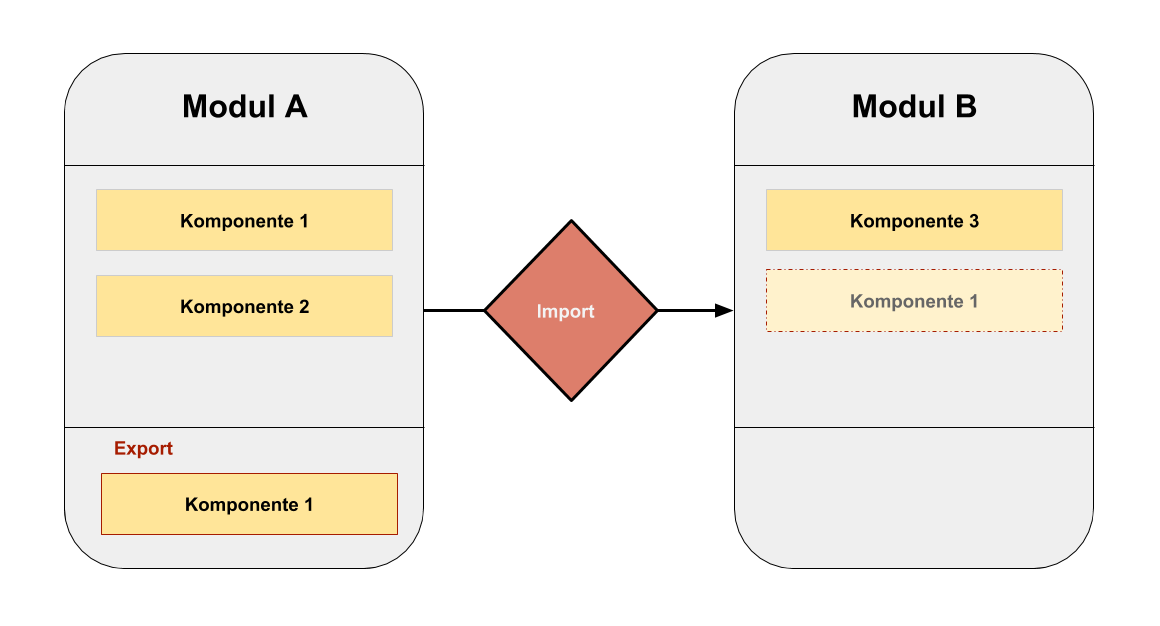
\epsfig{file = grundlagen/images/module.png, width=14.0cm}}
	\caption[Audi Konfigurator]{\textit{Fallbeispiel mit zwei Angular Modulen mit Komponenten}}
	\label{fig:ngModule}
\end{figure} 
%
Das hier beschriebene Beispiel ist in Abbildung \ref{fig:ngModule} zu sehen. Angenommen wir haben ein \textit{Modul A}. In diesem Modul sind nun \textit{Komponente 1} und \textit{Komponente 2} deklariert. Das heißt, es ist möglich in \textit{Komponente 1} die \textit{Kompontente 2} zu verwenden und umgekehrt, weil beide in dem \textit{Modul A} registriert sind. Jetzt haben wir ein weiteres \textit{Modul B}. In diesem ist die \textit{Komponente 3} registriert. Nun wäre es sehr praktisch, wenn \textit{Komponente 3} ebenfalls \textit{Komponente 1} aus dem anderen Modul verwenden könnte. Wie schon erwähnt darf ein Baustein in Angular nur in einem Modul registriert bzw. inititalisiert werden. Deshalb muss das \textit{Modul A} in \textit{Modul B} importiert werden, damit auch dort die \textit{Komponente 1} verwendet werden kann. Zusätzlich muss in \textit{Modul A} die \textit{Komponente 1} exportiert werden. Dadurch wird sie erst von außen frei zugänglich und somit in Bausteinen anderer Module nutzbar.
%
\paragraph{Hauseigene Module}
Angular hat auch ein paar hauseigene Module, die je nach Anwendungsfall importiert werden können. Das \textit{BrowserModule} wird für Web-Anwendungen im Angular-Umfeld genutzt und verfügt über alle Funktionalitäten, mit dem wir in der Lage sind, Ereignisse innerhalb des Browsers abzufangen, DOM-Rendering durchführen zu können und damit schließlich die lauffähige Angular-Anwendung im Browser realisieren zu können.\\
Das \textit{CommonModule} beinhaltet allgemeine Funktionen, die sehr, sehr häufig genutzt werden. Diese Funktionen liegen in Form von Direktiven und Pipes vor, womit ich bestimmen kann, ob ein HTML-Knoten angezeigt wird oder nicht oder auch Pipes, womit ich Ausgaben formatieren kann. Auch sprachabhängige Funktionalitäten sind in den \textit{CommonModule} enhalten.\\
Das \textit{HttpModule} ist dafür da, Client-Server-Kommunikation zu betreiben. Das heißt, HTTP-Requests lassen sich mit Hilfe des \textit{HttpModules} hervorragend realisieren, dafür werden Services zur Verfügung gestellt. Das \textit{HttpModule} hat auch Services für Testings und Co. Für Formulare gibt es entweder das FormsModule oder das \textit{ReactiveFormsModule}. Das hängt so ein wenig davon ab, wie man Formulare in der Anwendung gestalten will.\\
Das \textit{RouterModule} ist dafür da, um Komponenten-Routing zu realisieren. Das Routing ist die Grundlage für \textit{Single-Page-Applications}. Das heißt, über das Routing kann man bestimmen, welche Komponente dargestellt werden muss, wenn ein bestimmter Pfad in der Anwendung besucht wird.
%
\subsection{Grundfunktionen des Frameworks}
\label{subsec:grundfunktionen}
%
Module und Komponenten in Angular haben wir nun schon etwas ausführlicher betrachtet. Nun wollen wir uns weitere Funktionen und Bestandteile von Angular anschauen\footnote{Auf die weiteren Bestandteile von Angular wird hier nicht im Details eingegangen. Genauere Dokumentationen dazu sind online unter angular.io zu finden.}. Wie die einzelnen Bausteine umgesetzt und implementiert werden können sehen wir noch in Kapitel 4 Methodik am Fallbeispiel des 3D Konfigurators für Mehrwegbecher.
%
\paragraph{Bindungen}
%
\textit{\glqq Bindungen sind im Wesentlichen die Brücke zwischen der Darstellungsschicht und der Logikschicht\grqq } \cite{unlu_angular_2018}. Man kann beispielsweise Variablen oder Eigenschaften aus der TypeScript-Klasse in der Vorlage binden. Beispiel: Ich gebe die Variable \texttt{title} in der Vorlage als\texttt{ <h1> \{\{title\}\} </h1>} aus. Natürlich geht das ganze noch deutlich komplexer. Dadurch wird die Komponente mit ihrem Content dynamisch.
%
\paragraph{Direktiven}
%
Direktiven spielen innerhalb der Angular-Welt eine ähnlich wichtige Rolle wie Komponenten. Unter der Haube sieht man sogar, dass die voneinander erben. Im Wesentlichen ist es so, dass Direktiven in Vorlagen genutzt werden können. Und wie nutze ich sie? Indem ich Direktiven als Attribute auszeichne. Das heißt, Direktiven sind oft Attribute, die in ein HTML-Element hinzugefügt werden oder auch beispielsweise dadurch deklariert, dass an ein bestimmtes HTML-Element ein bestimmtes Attribut angehängt sein muss. Attribut-Direktiven machen eigentlich nichts anderes als eine Anpassung des Aussehens beziehungsweise eine Anpassung des Verhaltens eines Elements, das heißt, es manipuliert ein vorhandenes Element im Wesentlichen.\\
Analog dazu kann ich eine strukturelle Direktive in Form von ngFor benutzen. ngFor ist eine strukturelle Direktive, die etwas wahnsinnig Cleveres macht. Sie benutzt nämlich das Element, auf das sie angewendet wurde, als Vorlage, iteriert durch eine Liste, zum Beispiel eine unordered List, und packt diese Vorlage so oft in den DOM hinein, wie es Elemente in der Liste gibt.
%
\paragraph{Pipes}
%
Angular bietet uns die Möglichkeit zur Nutzung von Pipes. Sie dienen dazu, eine Ausgabe zu manipulieren. Überwiegend werden Pipes in Vorlagen genutzt.\\
Die Pipe manipuliert die Ausgabe und sorgt dafür, dass beispielsweise der Name in Großbuchstaben dargestellt wird. Analog lassen sich auch Pipes in Kette schalten. Das heißt, wenn ich eine Ausgabe habe, kann ich die wiederum in andere Pipes reinpacken.
%
\paragraph{Services}
%
Der Begriff Services in der Entwicklung ist so breit gefächert. Jede Programmiersprache versteht unter Services in gewissen Maßen was anderes. In der Angular-Welt sind Services Logiken, die allerdings View-unabhängig sind. Eine Komponente besteht aus Logik- und Darstellungsschicht, und in der Logikschicht habe ich ganz explizit die Logik, die nur für diese eine Komponente da ist.\\
Ein Service selber hat auch Logiken, die aber nicht allein für eine Komponente darstellen, sondern halt auch im Kontext in anderen Szenarien genutzt werden können. Super einfaches Beispiel dafür: Client-Server-Kommunikation. Wir können also einen Service erstellen, der das gesamte Handling des Logins steuert. Dieser Service verarbeitet dann via Passwort und Username die Client-Server-Kommunikation für das Login und empfängt vom Server dann das User-Objekt. Das kann aber an der anderen Stelle sein, dass ich zum Beispiel die Authentifizierung überprüfen möchte oder einfach nur das Geburtsjahr eines Users brauche, dann würde ich den gleichen Service in der anderen Komponente wieder nutzen und könnte dann entsprechend entweder auf die Eigenschaften des Services zurückgreifen, die es zuvor schon geholt hat, beziehungsweise auf Eigenschaftswerte, die es zuvor schon geholt hat, oder kann neue Requests triggern, Logger beispielsweise.
%
\subsection{Angular CLI}
Angular CLI ist ein mächtiges Tool. Es wird über die Command Line gesteuert. Sie kann beispielsweise verwendet werden, um ein neues Projekt anzulegen. Die CLI legt dann im Hintergrund die benötigte Projektstruktur mit allen benötigten Dateien in dem gewünschten Verzeichnis ab. Anschließend ist die Anwendung sogar schon lauffähig. Man kann sie ganz bequem über die CLI starten indem man den Developing Server verwendet. Mit Webpack wird das ganze Projekt gebündelt. Eine sehr große Hilfe können die Code Generatoren sein. Sie erzeugen uns automatisch Komponenten, Module oder Services. Dabei werden automatisch alle \texttt{@import-}Anweisungen vorgenommen. Wie das ganze konkret aussieht schauen wir uns bei der Umsetzung des Konfigurator noch einmal an. Angular bietet eine sehr gut verwendbare Testumgebung. Mit verschiedenen Modulen kann die Anwendung bis ins kleinste Detail getestet werden. Ganze User-Interaktionen können simuliert werden, auch auf verschiedenen Geräte-Klassifikationen. Wenn man die Anwendung veröffentlichen will, bietet das Framework über seine CLI eine build Funktion. Diese ermöglicht eine einfache und kompakte Lösung.
%
\subsection{Versionen}
Das Framework Angular setzt auf das System der semantischen Versionierung (\textit{SEMVER}). Die erste Version des Frameworks war \textit{AngularJS}. Schon die erste Version hatte das Ziel, ein strukturiertes und übersichtliches Framework zu sein. Mit der \textit{Version 2} wechselte die Programmiersprache von JavaScript zu TypeScript, welches von Microsoft entwickelt wurde. Das Framework wurde mit der Version 2 also komplett neu entwickelt. Es setzt aber großteils auf das alte Konzept von \textit{AngularJS}. Da das Router-Modul schon die Version 3 hatte, wurde die nächste Version von Angular komplett auf \textit{Version 4} angehoben, damit nun wieder alle Module auf der selben Version sind \cite{bohm_robin_angular_2017}. Mittlerweile ist die aktuelle Version des Framework \textit{Angular 7\footnote{Stand März 2019}}. Die aktuelle Version bringt ein paar Bugfixes mit sich sowie mehr Flexibilität. So können beispielsweise über die \textit{Angular CLI} ganz bequem alle Pakete automatisch aktualisiert werden. Anschließend sollte das Projekt mit der neuen Angular Version lauffähig sein (siehe \cite{steyer_ruhe_2018}).
%
%
%%%%%%%%%%%%%%%%%%%%%%%%%%%%%%%%%%%%%%%%%%%%%%%%%%%
%
% A U F B A U 
%
%%%%%%%%%%%%%%%%%%%%%%%%%%%%%%%%%%%%%%%%%%%%%%%%%%%
%
\section{Three.js}
\label{sec:three.js}
%
\textit{Die Entwicklung verbesserter 3D-Grafiken in webbasierten Anwendungen hat in letzter Zeit einen Schritt vorwärts getan, als Programmierer WebGL in die Mozilla Firefox Nightly-Builds und in WebKit integriert haben, das in Google Chrome und dem Safari-Browser von Apple verwendet wird. WebGL ist eine der am meisten entwickelten Bibliotheken, die von HTML5 unterstützt werden. }\cite{bahor_html5/webgl_2013}.\\
%
%
%%%%%%%%%%%%%%%%%%%%%%%%%%%%%%%%%%%%%%%%%%%%%%%%%%%
%
% A U F B A U 
%
%%%%%%%%%%%%%%%%%%%%%%%%%%%%%%%%%%%%%%%%%%%%%%%%%%%
%
\section{Responsive Webdesign}
\label{sec:responsive}
%
Der erste Eindruck ist wichtig. Ein Besucher benötigt nur 50 Millisekunden, um sich eine Meinung über eine Website zu bilden. Wenn also die Gestaltung der Webseite keinen guten ersten Eindruck hinterlässt, werden viele potenzielle Kunden einfach gehen\cite{webalive}. Laut einer Umfrage von \textit{clutch.co} sollen in 2019 nahezu alle Webseiten kleinerer Unternehmen mobil freundlich sein. Es ist offensichtlich, dass immer mehr mobile Geräte verwendet werden. Deshalb liegt es auch auf der Hand Webseiten für diese Geräteklasse anzupassen.
Laut einer Studie bevorzugen etwa 3/4 der Benutzer mobil freundliche Webseiten und würden sie auch wieder besuchen \cite{searchenginewatch}.\\
In seinem Artikel Responsive Web Design definiert Ethan Marcotte den Begriff mit 3 Säulen:\textit{ Flexible Layout-Grids, Flexible Bilder und Media Queries}. Er betont aber auch, dass es ein anderes Denken erfordert. \textit{Es ist ein mechanisches Konzept, das aus einer Person entsteht und auf endlichen, spezifischen Elementen basiert. Es gibt also keine klare Definition von Responsive Webdesign.} Oder anders gesagt: \textit{Ich kann Ihnen sagen, wie man Responsive Web Design macht. Wie wir die Dinge „reaktionsfähig“ machen, liegt an uns. Wir alle} \cite{responsive}.
%
%
%%%%%%%%%%%%%%%%%%%%%%%%%%%%%%%%%%%%%%%%%%%%%%%%%%%
%
% A U F B A U 
%
%%%%%%%%%%%%%%%%%%%%%%%%%%%%%%%%%%%%%%%%%%%%%%%%%%%
%
\section{Usability}
\label{sec:usability}
%
Usability ist ein umfassenderes Konzept, als allgemein unter „Benutzerfreundlichkeit“ oder „Benutzerfreundlichkeit“ verstanden wird. \\
Umfang, in dem ein System, ein Produkt oder eine Dienstleistung von bestimmten Benutzern verwendet werden kann, um bestimmte Ziele mit Effizienz, Effizienz und Zufriedenheit in einem bestimmten Nutzungskontext zu erreichen
Anmerkung 1 zum Begriff : Die „spezifizierten“ Benutzer, Ziele und Nutzungskontexte beziehen sich auf die bestimmte Kombination von Benutzern, Ziele und Nutzungskontext, für die die Verwendbarkeit in Betracht gezogen wird.
Anmerkung 2 zum Begriff : Das Wort „Usability“ wird auch als Qualifikationsmerkmal verwendet, um auf Designwissen, Kompetenzen, Aktivitäten und Designattribute zu verweisen, die zur Usability beitragen, wie beispielsweise Usability-Kenntnisse, Usability Professional, Usability Engineering, Usability-Methode, Usability-Bewertung Usability-Heuristik.
[QUELLE: ISO 9241-210: 2010, 2.13, geändert - Anmerkungen 1 und 2 wurden hinzugefügt.]
%
%
%%%%%%%%%%%%%%%%%%%%%%%%%%%%%%%%%%%%%%%%%%%%%%%%%%%
%
% A U F B A U 
%
%%%%%%%%%%%%%%%%%%%%%%%%%%%%%%%%%%%%%%%%%%%%%%%%%%%
%
\section{Performance}
\label{sec:performance}
%
\textit{Die Leistung vieler Websites hängt von der Auslastung der Website zu Spitzenzeiten unter verschiedenen Bedingungen ab. Leistungstests werden normalerweise in einer vernünftig simulierten Umgebung mit Hilfe von Leistungstestwerkzeugen durchgeführt. Die Leistung einer Website hängt jedoch von verschiedenen Parametern ab, und jeder Parameter muss unter verschiedenen Belastungsniveaus getestet werden.} Aufgrund der Komplexität von Websites ist es nicht möglich, einen gemeinsamen Nenner für Leistungsparameter zum Testen der Website zu zeichnen. Verschiedene Teile der Website müssen mit unterschiedlichen Parametern unter verschiedenen Bedingungen und Belastungsniveaus getestet werden. In solchen Fällen muss die Website in viele Komponenten zerlegt werden, die das Verhalten verschiedener Geschäftskomponenten darstellen. Diese Geschäftskomponenten werden verschiedenen Objekten zugeordnet, die das Verhalten und die Struktur des Teils der Website wirklich darstellen. Diese Objekte werden Leistungstests mit verschiedenen Parametern und Belastungsniveaus unterzogen. In diesem Dokument wird der neue Testprozess angesprochen, bei dem das Konzept der Zerlegung des Verhaltens der Website in testbare Komponenten verwendet wird, die auf testbare Objekte abgebildet werden. Diese überprüfbaren Objekte werden Leistungstests unter verschiedenen Leistungsparametern und Belastungsniveaus unterzogen.